\chapter{Path Planning Algorithms}%
\label{s_planning}

\section{Global A* Algorithm in Air Corridors}
\label{sec:astar_global}

For global path planning between vertiports, a graph search approach is adopted.
The urban airspace is modeled as an undirected, weighted graph where nodes
represent vertiports and edges represent available air corridors. The edge
weights are given by the geodesic distance between the connected vertiports,
computed using the Haversine formula. The planning objective is to determine the
shortest feasible route between a designated start and destination vertiport.

\subsection*{Problem Setup}
Let
\begin{itemize}
    \item $s \in V$ denote the starting vertiport,
    \item $d \in V$ denote the destination vertiport, and
    \item $n \in V$ denote a generic node (current vertiport) under expansion during the search.
\end{itemize}
The graph $G = (V,E)$ consists of a finite set of vertiports $V$ and undirected
edges $E \subseteq V \times V$, each edge $(u,v) \in E$ carrying a weight
$d(u,v)$ equal to the corridor distance between $u$ and $v$.

\subsection*{Illustration of the Search Graph}
\begin{figure}[H]
    \centering
    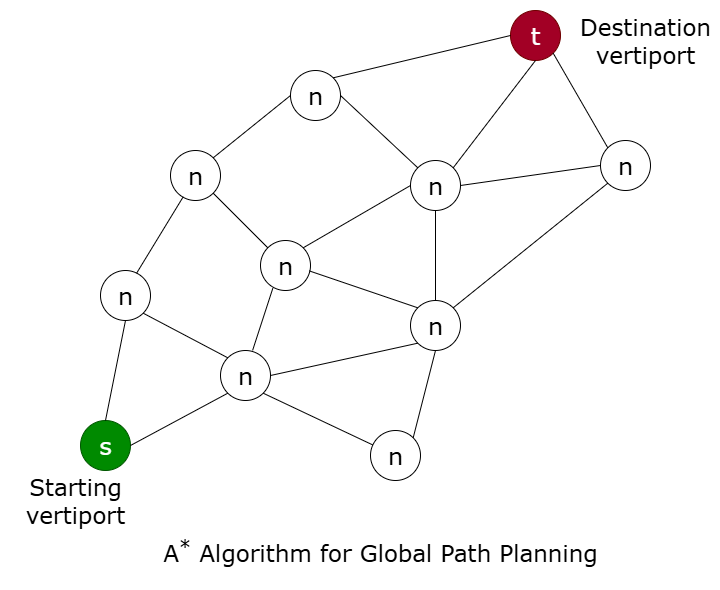
\includegraphics[width=0.6\textwidth]{figures/A_star.png}
    \caption{Illustration of the A* search on an undirected vertiport corridor graph.
    The starting node $s$ and destination node $d$ are connected through intermediate nodes $n$.}
    \label{fig:astar_graph}
\end{figure}

\subsection*{Heuristic}
To guide the A* search, the geodesic (Haversine) distance between the current
vertiport $n$ and the destination $d$ is used as the heuristic function $h(n)$.
Because the Haversine distance represents the shortest path on the Earth's
surface, it is admissible: the straight-line distance on the sphere is always
less than or equal to the length of any feasible path along the corridor
network.

Let $(\lambda_1,\varphi_1)$ and $(\lambda_2,\varphi_2)$ denote the longitude and
latitude (in radians) of the two points respectively. Define
$\Delta\varphi = \varphi_2 - \varphi_1$ and
$\Delta\lambda = \lambda_2 - \lambda_1$. Then the Haversine distance is given by

\begin{equation}
  d_\text{hav} = 2 R \arctan\!\Bigg(
  \frac{\sqrt{a}}{\sqrt{1-a}}\Bigg),
  \quad\text{with}\quad
  a = \sin^2\!\frac{\Delta\varphi}{2}
    + \cos\varphi_1 \cos\varphi_2
      \sin^2\!\frac{\Delta\lambda}{2},
\end{equation}

where $R$ is the Earth’s radius (here $R=\SI{6371}{km}$).

Accordingly, the heuristic function becomes
\begin{equation}
  h(n) = d_\text{hav}\big(\text{coord}(n), \text{coord}(d)\big),
\end{equation}
where $\text{coord}(v)$ denotes the geographic coordinates
$(\lambda,\varphi)$ of vertiport $v$.


\subsection*{Evaluation Function}
The total evaluation score for each node $n$ is defined as
\begin{equation}
    f(n) = g(n) + h(n),
\end{equation}
where $g(n)$ is the cumulative cost of the best-known path from $s$ to $n$, and
$h(n)$ is the heuristic estimate of the remaining cost to reach $d$.

In this context, the cost corresponds to the geodesic distance traveled along
the air corridors. Since the corridor network is assumed to operate at a fixed
altitude layer, the planning problem reduces to two dimensions, and the distance
is computed purely in terms of latitude and longitude. Thus, $g(n)$ accumulates
the 2D distances of all corridor segments from the start to the current node,
while $h(n)$ provides the straight-line (Haversine) estimate from the current
node to the destination. The evaluation score $f(n)$ therefore balances the actual
distance traveled so far with an optimistic estimate of the remaining distance,
ensuring efficient convergence toward the destination.

\subsection*{Algorithm}
The algorithm used is the classical A* search, adapted to the vertiport
corridor graph. It maintains a priority queue of nodes to be expanded,
ordered by their $f(n)$ value.

\begin{algorithm}[H]
\caption{A* Path Planning in Air Corridors}
\label{alg:astar}
\begin{algorithmic}[1]
\Require Start vertiport $s$, destination vertiport $d$, undirected graph $G = (V, E)$ with edge distances $d(u,v)$, coordinates $\text{coord}(v)$
\Ensure Sequence of vertiports representing the planned route
\State $open \gets \{s\}$ \Comment{priority queue with key $f(v)$}
\State $came\_from \gets \emptyset$
\State $g(s) \gets 0$
\State $f(s) \gets h(s) =$ Haversine$(\text{coord}(s), \text{coord}(d))$
\While{$open$ not empty}
  \State $current \gets \arg\min_{v \in open} f(v)$
  \If{$current = d$}
    \State \Return Reconstruct path from $came\_from$
  \EndIf
  \State Remove $current$ from $open$
  \ForAll{$neighbor \in$ neighbors($current$)}
    \State $tentative\_g \gets g(current) + d(current, neighbor)$
    \If{$tentative\_g < g(neighbor)$}
      \State $came\_from[neighbor] \gets current$
      \State $g(neighbor) \gets tentative\_g$
      \State $h(neighbor) \gets$ Haversine$(\text{coord}(neighbor), \text{coord}(d))$
      \State $f(neighbor) \gets g(neighbor) + h(neighbor)$
      \State Add $neighbor$ to $open$
    \EndIf
  \EndFor
\EndWhile
\State \Return failure (no path found)
\end{algorithmic}
\end{algorithm}

\subsection*{Output}
The algorithm returns the ordered list of vertiports
\begin{equation}
    \{ s, v_1, v_2, \dots, d \},
\end{equation}

that the aircraft should traverse. These nodes represent intermediate waypoints
along the air corridor network and form the global reference trajectory for
subsequent local planning and trajectory generation.

\section{Trajectory Generation Pipeline}
\label{s_traj_generation}

This section describes the generation of four–dimensional (4D) urban air mobility (UAM) trajectories
(latitude, longitude, altitude, time).This pipeline interfaces with the C++-based CFMS \cite{morscheck2021cfms} system while the planner is implemented in Python, demonstrating the microservice concept of this work. The pipeline transforms a discrete path over the vertiport
network into a kinematically consistent, phase–annotated trajectory by (i) synthesizing geometric
waypoints, (ii) assigning vertical and speed constraints, and (iii) invoking a modular flight
management and 4D trajectory generation system (CFMS) \cite{morscheck2021cfms} to densify and
time–parameterize the path.

\subsection{Notation and Conventions}
\label{s:traj_notation}

The following symbols and units are used throughout this work:
\begin{itemize}
  \item \textbf{Path over the graph:} $P = [v_0, v_1, \dots, v_n]$ is the ordered list of
  vertiports yielded by the global A* planner (Sec.~\ref{sec:astar_global}), with $v_0 = s$ (start)
  and $v_n = d$ (destination).

  \item \textbf{Coordinates:} each vertiport $v_i$ is associated with WGS–84 coordinates
  $\mathcal{V}(v_i) = (\varphi_i, \lambda_i, h_i)$ with
  latitude $\varphi_i$ (degrees), longitude $\lambda_i$ (degrees), and pad elevation $h_i$ (meters, MSL).

  \item \textbf{Altitude variables:} In this study, corridors are modelled at a fixed
    absolute altitude layer of \(H_{\text{corridor}}=\SI{200}{m}\) above mean sea level,
    independent of individual pad elevations. All cruise waypoints are therefore
    generated at this fixed altitude:
    \begin{equation}
        H^{\text{abs}} \;=\; H_{\text{corridor}}
    \end{equation}
    while take-off and landing waypoints use the actual pad elevation \(h_i\), and
    intermediate climb/descent waypoints interpolate between \(h_i\) and \(H_{\text{corridor}}\).

  \item \textbf{Time:} continuous time is denoted by $\tau$ (seconds). This symbol is used
  consistently in equations to represent elapsed time along a trajectory.

  \item \textbf{Geodesic distance:} $d(u,v)$ is the great-circle distance between two coordinates
  (Haversine).

  \item \textbf{Linear interpolation:} $\mathrm{lerp}(a,b,\alpha) \coloneqq a + (b-a)\,\alpha$, for $\alpha\in[0,1]$.
\end{itemize}


\subsection{Inputs}
The following inputs are used for the trajectory generation stage:

\begin{itemize}
  \item Path $P = [v_0, v_1, \dots, v_n]$ from A* (Sec.~\ref{sec:astar_global}).
  \item Vertiport map $\mathcal{V}: v_i \mapsto (\varphi_i, \lambda_i, h_i)$ (deg, deg, m MSL).
  \item Requested cruise height $H_c$ (AGL), default \SI{200}{m}.
  \item UAM speed profile with safety margin.
\end{itemize}

To ensure that the generated 4D trajectory remains flyable even under moderate disturbances 
(e.g.\ wind gusts, small deviations, or delayed responses), the nominal speeds used in this study 
are derived from the aircraft’s maximum performance values multiplied by a safety factor 
\(s_{\text{f}}\in(0,1)\).  
For the reference UAM vehicle the maximum performance limits are

\[
\begin{aligned}
    V_{\text{takeoff,max}}   &= \SI{0}{m/s}, \quad
    V_{\text{transition,max}} &= \SI{20}{m/s}, \\
    V_{\text{cruise,max}}     &= \SI{30}{m/s}, \quad
    V_{\text{approach,max}}   &= \SI{20}{m/s}.
\end{aligned}
\]

Applying a safety factor of \(s_{\text{f}}=0.75\) yields the nominal speeds adopted in the planning process:

\[
\begin{aligned}
    V_{\text{takeoff}}   &= s_{\text{f}}\;V_{\text{takeoff,max}} = \SI{0}{m/s}, \qquad
    V_{\text{transition}} &= s_{\text{f}}\;V_{\text{transition,max}} = \SI{15}{m/s},\\[0.5em]
    V_{\text{cruise}}    &= s_{\text{f}}\;V_{\text{cruise,max}} = \SI{25}{m/s}, \qquad
    V_{\text{approach}}  &= s_{\text{f}}\;V_{\text{approach,max}} = \SI{15}{m/s}.
\end{aligned}
\]


These safety-factored speeds are used as the target values for the 
\texttt{UAM\_takeoff}, \texttt{cruise} and \texttt{UAM\_landing} phases when 
annotating the waypoints.


\subsection{Waypoint Synthesis}
Given $P$, the waypoint generator produces an ordered list $W = [w_1,\dots,w_m]$ where each waypoint is
\begin{equation}
  w_k \;=\; \{\varphi_k, \lambda_k, H_k, \texttt{id}, \texttt{(optional) speed\_reduction}\}.
\end{equation}
The construction logic is as follows:
\begin{enumerate}
  \item \textbf{Initial takeoff point:} at $(\varphi_0,\lambda_0,h_0)$.
  \item \textbf{Mid–climb point:} along the initial bearing $v_0 \rightarrow v_1$ at
        \(\alpha=0.3\) of the segment, with altitude
        \begin{equation}
          H_{\text{climb}} \;=\; h_0 + 0.6\,(H^{\text{abs}} - h_0).
        \end{equation}
  \item \textbf{Cruise nodes at internal vertiports:} for each $v_i,\, i=1,\dots,n-1$,
        altitude is set to $H^{\text{abs}}$.
  \item \textbf{Pre–landing descent point:} along $v_{n-1} \rightarrow v_n$ at \(\alpha=0.7\)
        with
        \begin{equation}
          H_{\text{descent}} \;=\; h_n + 0.7\,(H^{\text{abs}} - h_n).
        \end{equation}
        This intermediate waypoint provides a clear transition from cruise altitude
        to the terminal approach. It produces a two-stage vertical profile
        (cruise $\rightarrow$ descent $\rightarrow$ landing) that smooths vertical-rate changes,
        yields more realistic trajectories, and leaves adequate horizontal distance
        for deceleration and stabilization before touchdown. The value
        \(\alpha=0.7\) is a simple, tunable heuristic chosen to begin the descent
        early enough for comfortable flare and speed control while preserving
        lateral fidelity.

  \item \textbf{Final landing point:} at $(\varphi_n,\lambda_n,h_n)$.
\end{enumerate}


\subsection{Phase Encoding and Speed Constraints}
Each waypoint is annotated with a nominal flight phase and target speed:

\begin{description}
  \item[\texttt{UAM\_takeoff}] Initial (pad) waypoint, executed at the takeoff speed \(V_{\text{takeoff}}\).
  \item[\texttt{cruise}] Mid–climb, internal cruise nodes, and descent–initiation nodes,
  with \(V_{\text{transition}}\) applied at climb/descent anchors and \(V_{\text{cruise}}\) along the en-route segments.
  \item[\texttt{UAM\_landing}] Final (pad) waypoint, with the speed set to \(0\,\text{m/s}\) (stationary at landing).
\end{description}


\subsection{CFMS Integration}
The waypoint list is converted to the CFMS input structure:
\begin{itemize}
  \item $(\varphi,\lambda)$ converted from degrees to radians.
  \item Altitudes expressed in meters MSL (using $H^{\text{abs}}$ for cruise waypoints).
  \item Phase and speed fields set as above; the global context specifies the aircraft type
  \texttt{CFMS\_UAMcopter}, cruise height $H_c$, and cruise speed $V_{\text{cruise}}$.
\end{itemize}
CFMS \cite{morscheck2021cfms} then generates a dense 4D trajectory
\(\mathcal{T} = \{(\varphi(\tau), \lambda(\tau), H(\tau), \tau, \dots)\}\) that satisfies the kinematic
profile and phase schedule.

\subsection{Temporal and Spatial Sampling}
To reduce data volume, the CFMS output is uniformly sub–sampled to at most $M=500$ points:
\begin{equation}
  \mathrm{index}_i \;=\; \left\lfloor \frac{i\,(N-1)}{M-1} \right\rfloor,\quad i=0,\dots,M-1,
\end{equation}
with $N$ original samples; the first and last samples are always retained.

\subsection{Exported Data Fields}
Each trajectory is represented as a sequence of sampled data points of the form
\begin{equation}
\{\varphi,\lambda,H,\texttt{t},\text{TAS},V_g,\phi,\dot{H},\dot{\psi},\texttt{flight\_phase}\},
\end{equation}
where:
\begin{itemize}
  \item $\varphi$ – latitude of the sample point (deg).
  \item $\lambda$ – longitude of the sample point (deg).
  \item $H$ – altitude above mean sea level (m).
  \item \texttt{t} – elapsed time since the start of the trajectory (s); denoted by $\tau$ in the equations.
  \item \text{TAS} – true airspeed (m/s): the speed of the vehicle relative to the surrounding air.
  \item $V_g$ – ground speed (m/s): magnitude of the velocity vector relative to the ground.
  \item $\phi$ – bank angle (deg): roll about the longitudinal axis; zero is wings-level.
  \item $\dot{H}$ – climb rate (m/s): time derivative of altitude; positive in climb, negative in descent.
  \item $\dot{\psi}$ – turn rate (deg/s): rate of change of the ground-track angle.  
  In coordinated flight it can be approximated by
  \begin{equation}
    \dot{\psi} \;=\; \frac{g\,\tan\phi}{V_g},
  \end{equation}
  where $g$ is gravitational acceleration (m/s$^2$).
  \item \texttt{flight\_phase} – label indicating the nominal phase of flight:
    \texttt{UAM\_takeoff} (departure and climb), 
    \texttt{cruise} (en-route), 
    \texttt{UAM\_landing} (approach and landing), or 
    \texttt{other} (any intermediate or internal phase).
\end{itemize}


\subsection{Algorithm Summary}
\begin{algorithm}[H]
\caption{Trajectory Generation from A* Path}
\label{alg:traj_gen}
\begin{algorithmic}[1]
\Require Path $P=[v_0,\dots,v_n]$, vertiport map $\mathcal{V}$, cruise height $H_c$ (AGL)
\Ensure Subsampled, phase–annotated 4D trajectory $\mathcal{T}'$
\State $H^{\text{abs}} \gets h_0 + H_c$ \Comment{constant cruise layer above departure pad}
\State $W \gets$ synthesize\_waypoints$(P,\mathcal{V},H^{\text{abs}})$
\State annotate phases and speeds in $W$ (\texttt{UAM\_takeoff}, \texttt{cruise}, \texttt{UAM\_landing})
\State $W_{\text{CFMS}} \gets$ convert\_to\_CFMS$(W)$ \Comment{radians; altitudes in m MSL}
\State $\mathcal{T} \gets$ CFMS\_generate\_trajectory$(W_{\text{CFMS}})$
\State $\mathcal{T}' \gets$ uniform\_subsample$(\mathcal{T}, M=500)$
\State export $\mathcal{T}'$ as JSON $\{\varphi,\lambda,H,\texttt{t},\dots\}$
\end{algorithmic}
\end{algorithm}

\paragraph{Consistency with Global Planning.}
The global A* planner (Sec.~\ref{sec:astar_global}) minimizes 2D geodesic distance over the corridor
graph at a fixed altitude layer. The trajectory pipeline respects this assumption by assigning a
constant cruise height $H_c$ (AGL) along the route and applying geodesic distances only for horizontal planning.

\section{Conflict Detection with NDMap}
\label{sec:ndmap}

The following section is a summarized version of the NDMap conflict detection method presented in \cite{NDMap}, adapted to the requirements of this work.

\subsection*{Overview}
In this work, conflicts are detected using NDMap configured in four dimensions
\((\lambda,\varphi,H,\tau)\), i.e., longitude \([\mathrm{deg}]\), latitude \([\mathrm{deg}]\), altitude \([\mathrm{m}]\), and time \([\mathrm{s}]\).
NDMap indexes submitted trajectories in this 4D space and, for a newly inspected trajectory,
efficiently identifies portions of previously submitted trajectories that come within
user-defined separation minima. This enables very fast screening suitable for near real-time admission control.

\subsection*{Inputs and Configuration}
Each trajectory is represented as an ordered sequence of sampled four-dimensional points
\[
(\lambda,\varphi,H,\tau)
\;\in\;
[-180^\circ,180^\circ] \times [-90^\circ,90^\circ] \times [0,100000]~\text{m} \times [0,86400]~\text{s},
\]
where  
$\lambda$ is longitude (deg),  
$\varphi$ is latitude (deg),  
$H$ is altitude above mean sea level (m), and  
$\tau$ is time (s).

Separation requirements are encoded as a vector
\begin{equation}
  \mathbf{S} \;=\; 
  \bigl(\Delta\lambda_{\min},\,\Delta\varphi_{\min},\,\Delta H_{\min},\,\Delta\tau_{\min}\bigr),
\end{equation}
which sets the minimum allowed spacing in each dimension and parameterizes the detector’s resolution.  
In this study,
\[
\mathbf{S} = 
\bigl(0.002^\circ,\;0.004^\circ,\;300~\text{m},\;90~\text{s}\bigr),
\]
corresponding respectively to minimum separations in longitude (deg), latitude (deg), altitude (m), and time (s).  
A minimum inter-conflict interval of \(2~\text{s}\) is applied to merge very closely spaced detections.

\subsection*{Output}
For each conflicting pair involving the inspected trajectory, NDMap returns one or more
\emph{conflict time intervals}
\[
[\tau_{\text{start}},\,\tau_{\text{end}}],
\]
expressed in seconds on the scenario time axis. These intervals constitute the primary output consumed
by the deconfliction/scheduling logic in this work.

\subsection*{Performance Characteristics}
According to the NDMap documentation \cite{NDMap}, runtimes are on the order of
milliseconds per trajectory on commodity hardware, with reported averages of a few milliseconds per
object for national- to continental-scale datasets. The implementation exhibits near-linear scaling
with dataset size and tunable trade-offs between runtime and memory via configuration parameters, which
supports near real-time screening in the intended UAM use case.

\medskip
\noindent\textbf{Summary.}
NDMap consumes sampled 4D trajectories together with separation minima \(\mathbf{S}\) and produces
conflict time intervals \([\tau_{\text{start}},\tau_{\text{end}}]\) for any violations. The detector’s
low latency and favorable scaling make it appropriate for iterative, online conflict checks within
the planning pipeline described in this thesis.

\section{Conflict Resolution}
\label{sec:conflict_resolution}

Conflict detection with NDMap (Sec.~\ref{sec:ndmap}) identifies spatio-temporal overlaps 
between a newly proposed candidate trajectory and the set of already submitted trajectories. 
To ensure conflict-free operation, conflict resolution is applied directly within the 
path planning loop of this work.

\subsection*{Resolution Strategy}
In this study, conflict resolution is realized through \textbf{lateral re-routing}. 
The principle is to discourage the reuse of route segments that are involved in conflicts 
and to force the planner to search for an alternative path through the corridor network.

\begin{enumerate}
    \item A candidate path is computed using the global A* planner (Sec.~\ref{sec:astar_global}).
    \item The corresponding trajectory is generated and checked against existing traffic using NDMap.
    \item If a conflict is detected, the edges of the corridor graph that belong to the conflicting candidate route are penalized by 
    assigning them effectively infinite weight, i.e.,
    \[
      d(u,v) \;\coloneqq\; \infty, \quad \forall\,(u,v)\in E_{\text{conflict}},
    \]
    which removes them from further consideration by A*.
    \item A* is re-executed on the modified graph to find an alternative route that avoids the discouraged edges.
    \item This process is repeated iteratively until NDMap no longer reports conflicts.
\end{enumerate}

\subsection*{Properties}
This integrated resolution approach has the following characteristics:
\begin{itemize}
    \item \textbf{Simplicity:} implemented as an extension of the global A* search without requiring additional modules.
    \item \textbf{Determinism:} the iterative penalization guarantees that once all conflicting edges are discouraged, 
    the resulting solution is conflict-free (if a feasible route exists).
    \item \textbf{Cost trade-off:} since conflicts are avoided by forbidding certain edges, 
    the resulting route may be longer than the original candidate, reflecting a trade-off between efficiency and safety.
    \item \textbf{Scalability:} the conflict detection and re-routing loop can be repeated for successive trajectory submissions, 
    enabling online admission control in multi-UAV settings.
\end{itemize}

\subsection*{Scope of this Work}
Although other resolution mechanisms such as temporal shifting or vertical maneuvering 
are possible, the present work focuses exclusively on lateral re-routing within the 
corridor graph. This allows for a modular and scalable demonstration of how conflict 
detection (via NDMap) and path planning (via A*) can be tightly integrated in a unified framework.

\begin{figure}[H]
    \centering
    \begin{subfigure}{0.45\textwidth}
        \centering
        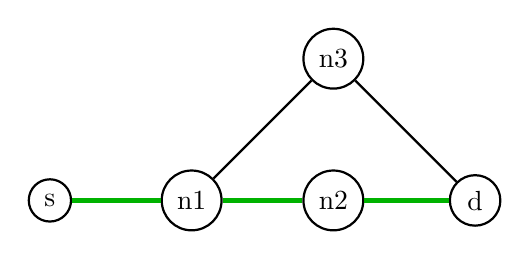
\begin{tikzpicture}[node distance=1.8cm,thick]
            % Nodes
            \node[circle,draw] (s) {s};
            \node[circle,draw,right of=s] (a) {n1};
            \node[circle,draw,right of=a] (b) {n2};
            \node[circle,draw,right of=b] (d) {d};
            \node[circle,draw,above of=b] (c) {n3};

            % Edges
            \draw (s) -- (a);
            \draw (a) -- (b);
            \draw (b) -- (d);
            \draw (a) -- (c) -- (d);

            % Path
            \draw[green!70!black,ultra thick] (s) -- (a) -- (b) -- (d);
        \end{tikzpicture}
        \caption{Initial candidate path (green).}
    \end{subfigure}
    \hfill
    \begin{subfigure}{0.45\textwidth}
        \centering
        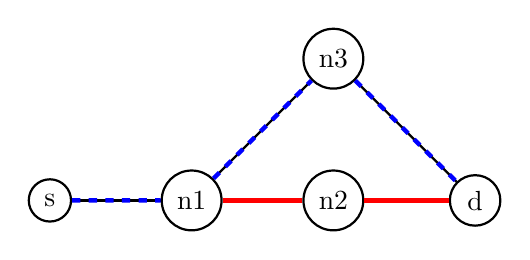
\begin{tikzpicture}[node distance=1.8cm,thick]
            % Nodes
            \node[circle,draw] (s) {s};
            \node[circle,draw,right of=s] (a) {n1};
            \node[circle,draw,right of=a] (b) {n2};
            \node[circle,draw,right of=b] (d) {d};
            \node[circle,draw,above of=b] (c) {n3};

            % Edges
            \draw (s) -- (a);
            \draw (a) -- (b);
            \draw (b) -- (d);
            \draw (a) -- (c) -- (d);

            % Conflict edges
            \draw[red,ultra thick] (a) -- (b);
            \draw[red,ultra thick] (b) -- (d);

            % New path
            \draw[blue,ultra thick,dashed] (s) -- (a) -- (c) -- (d);
        \end{tikzpicture}
        \caption{Conflict edges penalized (red), re-routed path (blue dashed).}
    \end{subfigure}
    \caption{Illustration of conflict resolution via lateral re-routing.}
    \label{fig:conflict_resolution}
\end{figure}


